%-------------------------------------------------------------------------
% PACKAGES AND OTHER DOCUMENT CONFIGURATIONS
%-------------------------------------------------------------------------

\documentclass[11pt]{article}
%----------------------------------------------------------------------------------------------
%   PACKAGES AND CONFIGURATIONS 
%----------------------------------------------------------------------------------------------

\usepackage{lastpage}
\usepackage{hyperref}
\usepackage{graphicx}
\usepackage{pgfplots}
\pgfplotsset{compat=1.17}
\usepackage{xcolor}
\usepackage{amsmath}
\usepackage{bussproofs}
\usepackage{amssymb}
\usepackage{amsfonts}
\usepackage{graphicx}
\usepackage{booktabs}
\usepackage{listing}
\usepackage{etoolbox}
\usepackage{latexsym}
\usepackage{listings}
\usepackage[utf8]{inputenc}
\usepackage{caption}
\graphicspath{{./img}}

\DeclareCaptionFont{white}{\color{white}}
\DeclareCaptionFormat{listing}{%
  \parbox{\textwidth}{\colorbox{gray}{\parbox{\textwidth}{#1#2#3}}\vskip-4pt}}
\captionsetup[lstlisting]{format=listing,labelfont=white,textfont=white}
\lstset{frame=lrb,xleftmargin=\fboxsep,xrightmargin=-\fboxsep}

%-----------------------------------------------------------------------------------------------
%   MARGINS
%-----------------------------------------------------------------------------------------------

\usepackage{geometry}
\geometry{
    paper=a4paper,
    top=3cm,
    bottom=3cm,
    left=2.5cm,
    right=2.5cm,
    headheight=14pt,
    footskip=1.4cm,
    headsep=1.2cm,
}

%-----------------------------------------------------------------------------------------------
%   FONT
%-----------------------------------------------------------------------------------------------

\usepackage[utf8]{inputenc}
\usepackage[T1]{fontenc}

\usepackage[sfdefault,light]{roboto}

%-----------------------------------------------------------------------------------------------
%   HEADER AND FOOTER   
%-----------------------------------------------------------------------------------------------

\usepackage{fancyhdr}
\pagestyle{fancy}

\lhead{\small\classHomework\ifdef{\className}{\ (\className):}{}\ \homeworkTitle}
\chead{}
\rhead{\small\ifdef{\authorName}{\authorName}{\ifdef{dueDate}{Due\ \dueDate}{}}}

\lfoot{}
\cfoot{\small Page\ \thepage\ of\ \pageref{LastPage}}
\rfoot{
\includegraphics[scale=0.06]{logo-unige.png}}

\renewcommand\headrulewidth{0.5pt}

%-------------------------------------------------------------------------------------------------
%   TITLE PAGE
%-------------------------------------------------------------------------------------------------

\author{\textbf{\authorName}}
\date{}

\title{
    \thispagestyle{empty}
    \vspace{0.2\textheight}
    \textbf{\classHomework:\ \homeworkTitle}\\[-4pt]
    \ifdef{\classHomework}{{\small Due\ on\ \dueDate}\\}{}
    \ifdef{\className}{{\large \textit{\className}}}{}
    \vspace{0.32\textheight}

    
\includegraphics[scale=0.2]{logo-unige.png}
}
 % Ensure this file contains all necessary package inclusions and settings

%-------------------------------------------------------------------------
% HOMEWORK INFORMATION
%-------------------------------------------------------------------------

\newcommand{\classHomework}{13X007}
\newcommand{\homeworkTitle}{Assignment\ \#7}
\newcommand{\authorName}{CHRISTOFOROU Anthony}
\newcommand{\className}{Parallelism}
\newcommand{\dueDate}{30.11.2023}

%-------------------------------------------------------------------------

\begin{document}
    
    \maketitle
    \thispagestyle{empty}
    \newpage

    \tableofcontents
    
    \newpage
    
    \hypertarget{introduction}{%
    \section{Introduction}\label{introduction}}

    This comprehensive report delves into the performance analysis of a heat
    simulation application, deployed on diverse hardware setups. We
    scrutinize the application on Yggdrasil High-Performance Computing (HPC)
    with an array of 32 CPUs and a GPU, juxtaposed against its performance
    on a personal computer equipped with 12 CPU cores and an NVIDIA RTX 2070
    Super GPU. The crux of this analysis lies in discerning the execution
    time disparities when run on CPU versus GPU.

    \hypertarget{methodology}{%
    \section{Methodology}\label{methodology}}

    \hypertarget{hardware-employed}{%
    \subsection{Hardware Employed}\label{hardware-employed}}

    \begin{itemize}
    
    \item
    \textbf{Yggdrasil HPC:} A formidable configuration of 32 CPUs
    alongside a single GPU.
    \item
    \textbf{Personal Computer:} A setup comprising 12 CPU cores and an RTX
    2070 Super GPU.
    \end{itemize}

    \hypertarget{software-and-compilation}{%
    \subsection{Software and Compilation}\label{software-and-compilation}}

    \begin{itemize}
    
    \item
    The application is compiled using \texttt{g++} for CPU-centric
    execution, and \texttt{nvcc}, NVIDIA's CUDA compiler, for GPU
    execution.
    \item
    The incorporation of the Threading Building Blocks (TBB) library
    (\texttt{-ltbb}) hints at the application's potential for
    multi-threaded operations on the CPU.
    \end{itemize}

    \hypertarget{results}{%
    \section{Results}\label{results}}

    \hypertarget{performance-metrics}{%
    \subsection{Performance Metrics}\label{performance-metrics}}

    \begin{enumerate}
    \def\labelenumi{\arabic{enumi}.}
    
    \item
    \textbf{On Yggdrasil HPC:}

    \begin{itemize}
    
    \item
        \textbf{CPU (32 cores):} Marked an execution time of 4,139,176
        microseconds.
    \item
        \textbf{GPU:} Recorded an execution time of 5,800,258 microseconds.
    \end{itemize}
    \item
    \textbf{On Personal Computer:}

    \begin{itemize}
    
    \item
        \textbf{CPU (12 cores):} Notched an execution time of 2,653,190
        microseconds.
    \item
        \textbf{GPU (RTX 2070 Super):} Clocking in at 2,652,420
        microseconds.
    \end{itemize}
    \end{enumerate}

    \newpage

    \hypertarget{graphical-representation}{%
    \section{Graphical Representation}\label{graphical-representation}}

    A bar graph vividly depicts the execution times, contrasting the
    performance across the varied hardware configurations.

    \begin{figure}[ht]
    \centering
    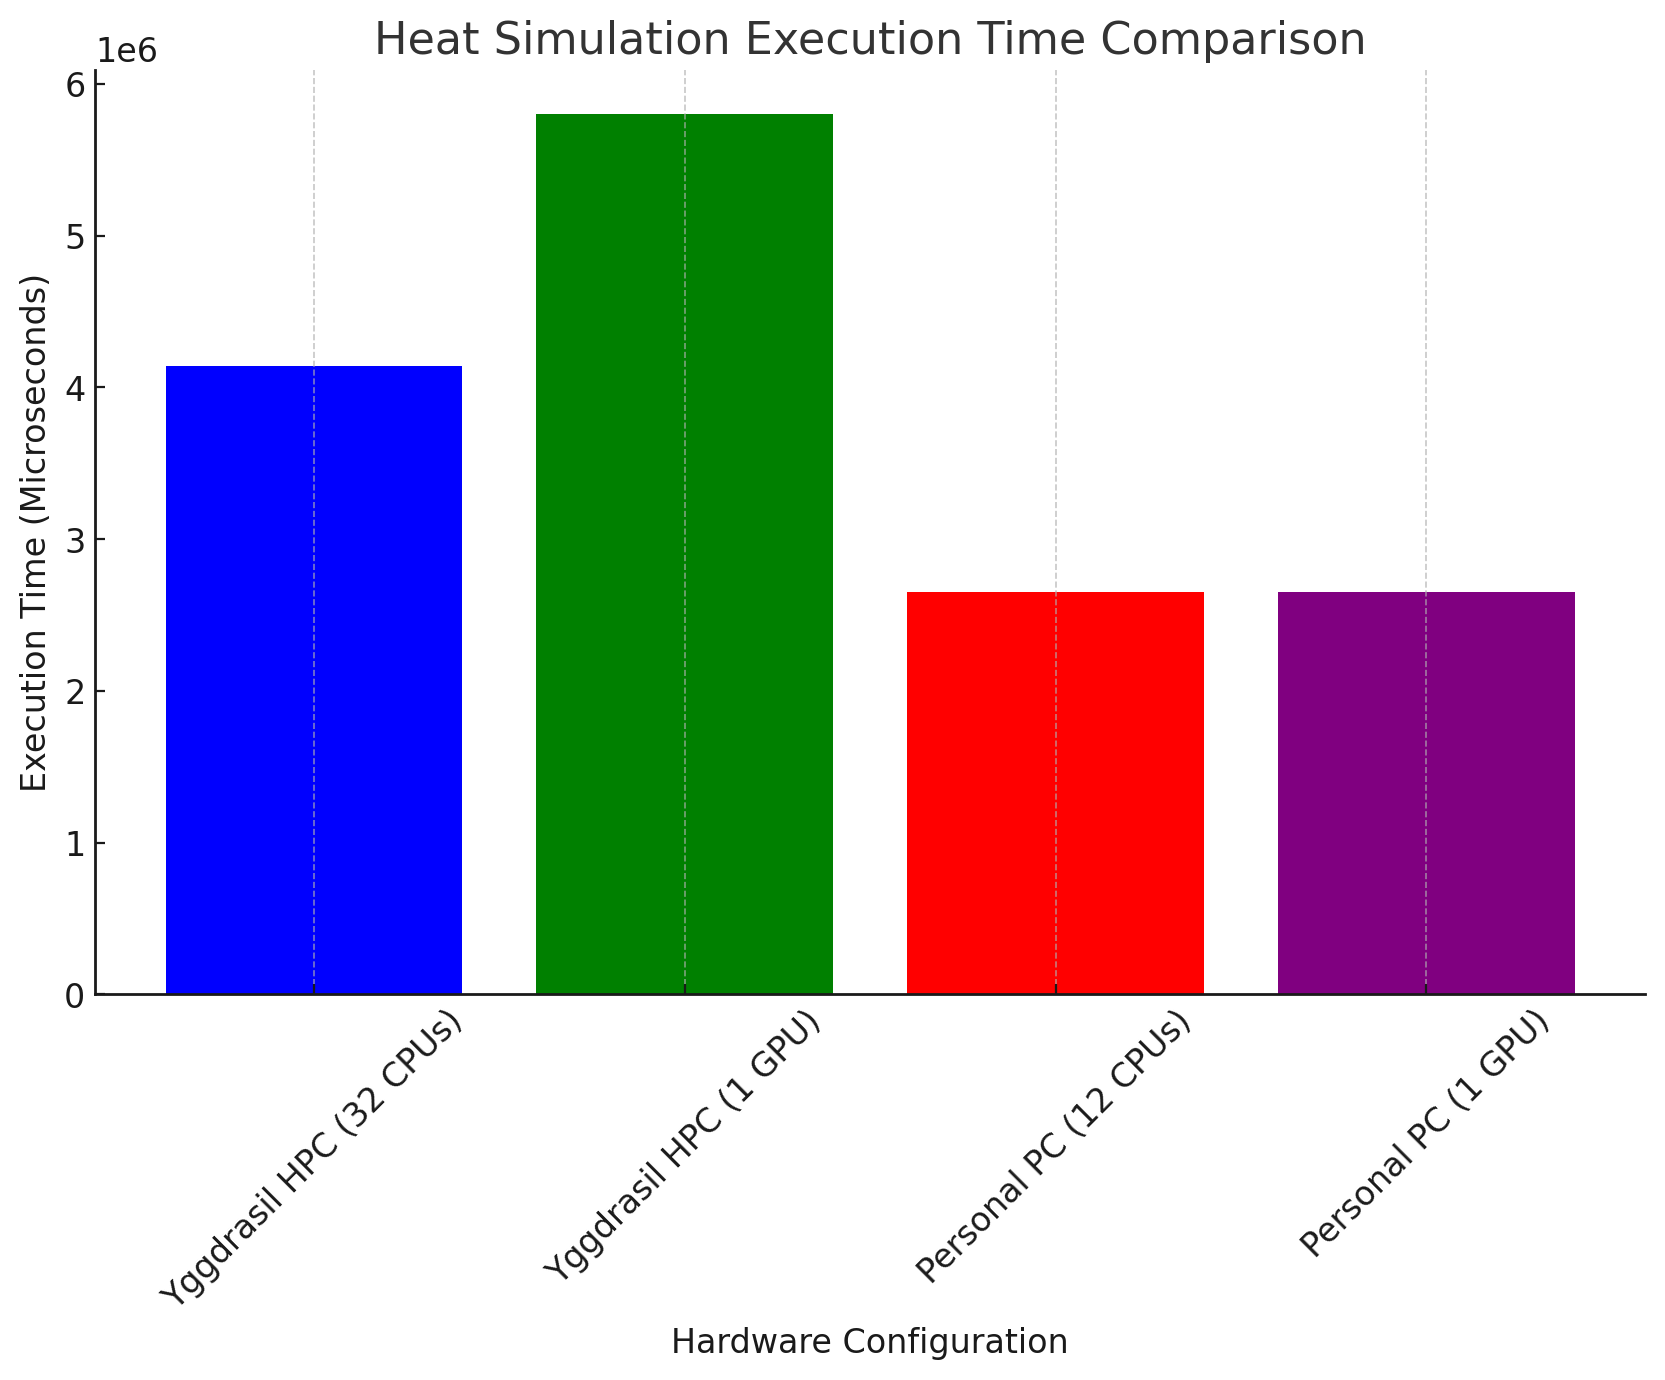
\includegraphics[width=0.8\textwidth]{img/execution_time.png}
    \caption{Execution Times}
    \end{figure}

    \hypertarget{analysis-of-code}{%
    \section{Analysis of Code}\label{analysis-of-code}}

    \hypertarget{cpu-implementation}{%
    \subsection{CPU Implementation}\label{cpu-implementation}}

    \begin{itemize}
    
    \item
    The code harnesses an array of standard C++ libraries for various
    functionalities, ranging from input/output operations to mathematical
    computations and parallel execution capabilities.
    \item
    Key constants like \texttt{max\_iter}, \texttt{Nx}, and \texttt{Ny}
    are pivotal in setting the simulation parameters.
    \item
    The vectors \texttt{U} and \texttt{U0} are instrumental in
    representing the state of the simulation grid.
    \item
    The simulation loop leverages \texttt{std::for\_each} combined with
    \texttt{std::execution::par\_unseq}, optimizing for parallel execution
    across CPU cores.
    \item
    Timing metrics are meticulously captured using
    \texttt{high\_resolution\_clock}, providing granular insights into
    execution efficiency.
    \end{itemize}

    \hypertarget{gpu-implementation}{%
    \subsection{GPU Implementation}\label{gpu-implementation}}

    \begin{itemize}
    
    \item
    The specifics of GPU optimization and parallel processing remain
    elusive in the provided code snippet, leaving room for speculation
    about its execution efficiency and optimization on the GPU front.
    \end{itemize}

    \hypertarget{discussion}{%
    \section{Discussion}\label{discussion}}

    \hypertarget{performance-insights}{%
    \subsection{Performance Insights}\label{performance-insights}}

    \begin{itemize}
    
    \item
    \textbf{Personal Computer:} The performance metrics interestingly
    reveal that the GPU, despite having fewer cores than the CPU, delivers
    comparable execution efficiency.
    \item
    \textbf{Yggdrasil HPC:} The CPU's performance notably eclipses that of
    the GPU, indicating more effective utilization of resources or
    possibly superior parallel processing capabilities in this scenario.
    \end{itemize}

    \hypertarget{factors-influencing-performance}{%
    \subsection{Factors Influencing
    Performance}\label{factors-influencing-performance}}

    \begin{itemize}
    
    \item
    \textbf{CPU Efficiency:} The application's CPU version exhibits
    impressive multi-threading efficiency, particularly on the HPC's
    multi-core setup.
    \item
    \textbf{GPU Limitations:} GPU performance could be hindered by factors
    like memory transfer bottlenecks and less optimized kernel execution,
    particularly evident in the HPC environment.
    \end{itemize}

    \hypertarget{potential-for-optimization}{%
    \subsection{Potential for
    Optimization}\label{potential-for-optimization}}

    \begin{itemize}
    
    \item
    Both CPU and GPU implementations present opportunities for
    enhancement. Optimizing memory access patterns, refining thread
    management, and fine-tuning kernel execution parameters for GPUs are
    potential areas for improvement.
    \end{itemize}

    \hypertarget{conclusion}{%
    \section{Conclusion}\label{conclusion}}

    The report meticulously evaluates the performance of a heat simulation
    application across various hardware settings, uncovering valuable
    insights into its operational dynamics. The findings gleaned from this
    analysis serve as a cornerstone for strategizing optimizations tailored
    to high-performance computing applications.

    
\end{document}
